\documentclass[border=12pt]{standalone}
\usepackage{tikz}
\usetikzlibrary{arrows.meta, positioning}
\usepackage{amsmath, amssymb}

\begin{document}
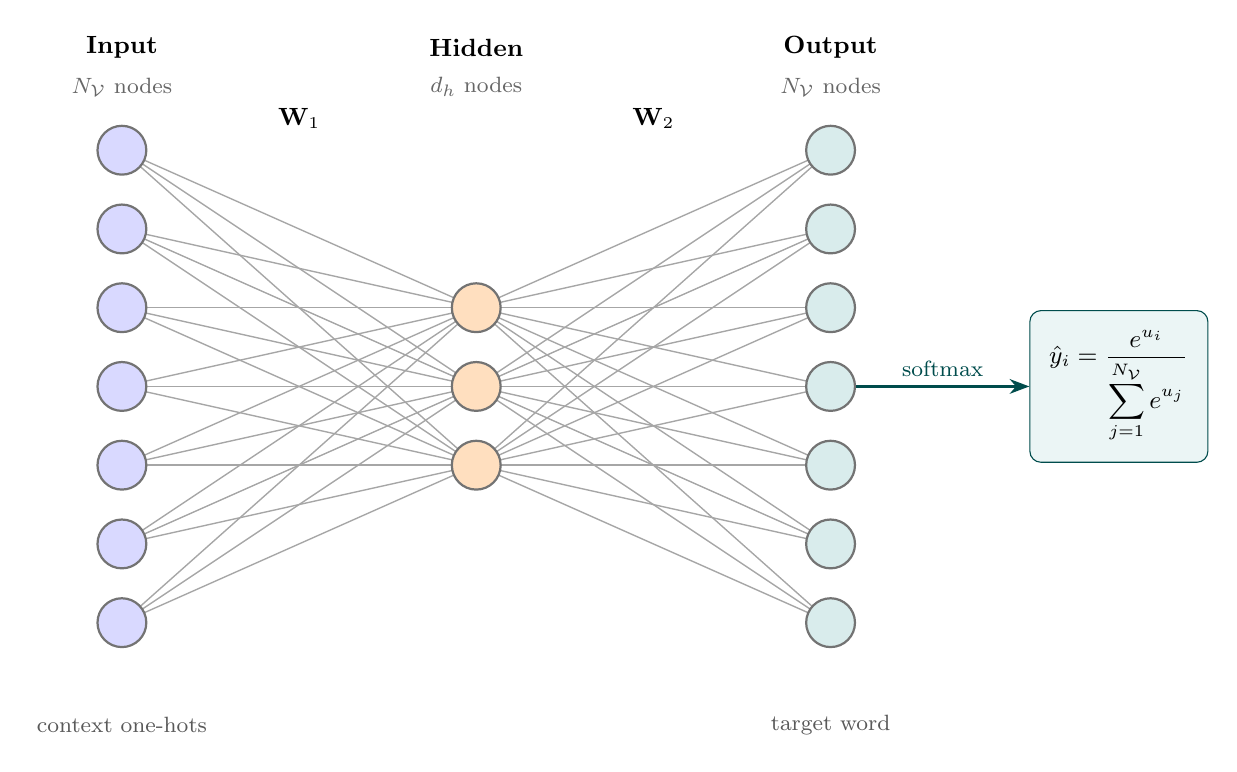
\begin{tikzpicture}[
    neuron/.style = {circle, draw=black!55, thick, minimum size=0.62cm, inner sep=0pt},
    inp/.style    = {neuron, fill=blue!15},
    hid/.style    = {neuron, fill=orange!25},
    outp/.style   = {neuron, fill=teal!15},
    conn/.style   = {draw=gray!70, line width=0.5pt},
    arr/.style    = {-{Stealth[length=2.5mm]}, thick},
]

%% ---- Edges first so neurons sit on top ----

% input -> hidden
\foreach \i in {1,...,7}{
    \foreach \h in {1,...,3}{
        \draw[conn] (0, {4-\i}) -- (4.5, {2-\h});
    }
}

% hidden -> output
\foreach \h in {1,...,3}{
    \foreach \o in {1,...,7}{
        \draw[conn] (4.5, {2-\h}) -- (9.0, {4-\o});
    }
}

%% ---- Neurons ----

\foreach \i in {1,...,7}{ \node[inp] (I\i) at (0,   {4-\i}) {}; }
\foreach \h in {1,...,3}{ \node[hid] (H\h) at (4.5, {2-\h}) {}; }
\foreach \o in {1,...,7}{ \node[outp] (O\o) at (9.0, {4-\o}) {}; }

%% ---- Layer headers ----

\node[font=\small\bfseries]         at (0.0, 4.3) {Input};
\node[font=\footnotesize, black!60] at (0.0, 3.8) {$N_{\mathcal{V}}$ nodes};

\node[font=\small\bfseries]         at (4.5, 4.3) {Hidden};
\node[font=\footnotesize, black!60] at (4.5, 3.8) {$d_h$ nodes};

\node[font=\small\bfseries]         at (9.0, 4.3) {Output};
\node[font=\footnotesize, black!60] at (9.0, 3.8) {$N_{\mathcal{V}}$ nodes};

%% ---- W1 / W2 labels: placed above the connection fans, no fill, no draw ----

\node[font=\small] at (2.25, 3.4) {$\mathbf{W}_1$};
\node[font=\small] at (6.75, 3.4) {$\mathbf{W}_2$};

%% ---- Context and target labels below the columns ----

\node[font=\footnotesize, black!65, align=center] at (0.0, -4.3) {context one-hots};
\node[font=\footnotesize, black!65, align=center] at (9.0, -4.3) {target word};

%% ---- Softmax box ----

\node[draw=teal!60!black, rounded corners=4pt, fill=teal!8, font=\small,
      right=2.2cm of O4, align=center, inner sep=7pt] (sfx)
    {$\hat{y}_{i} = \dfrac{e^{u_i}}{\displaystyle\sum_{j=1}^{N_{\mathcal{V}}} e^{u_j}}$};

\draw[arr, teal!60!black] (O4.east) -- (sfx.west)
    node[midway, above, font=\footnotesize] {softmax};

\end{tikzpicture}
\end{document}
